\begin{center}
	{\bf\normalsize Демонстрация работы программы}
\end{center}

В обработчике прерывания отдельно обрабатывается BackSpace и Shift.

В случае BackSpace последний перед курсором символ стирается.

В случае Shift происходит смена регистра и печатается '*'.



В начале программа стартует в реальном режиме и ждёт нажатия любой клавиши для перехода:

\begin{figure}[!ht]
	\begin{center}
		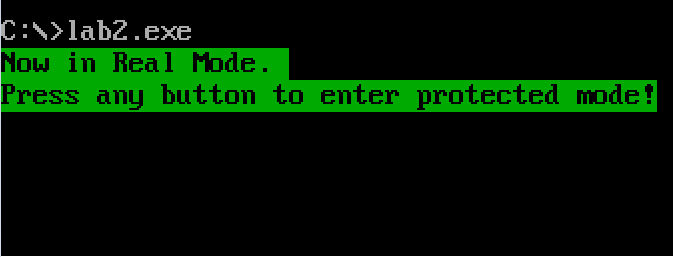
\includegraphics[width=16cm]{inc/start.png}
	\end{center}
\end{figure}

После перехода в защищённый режим программа подсчитывает количество доступной памяти и выводит значение на экран.
При этом справа от значения есть квадрат, который постоянно меняет свой цвет по тику.
Снизу пользователь может вводить символы на экран:

\begin{figure}[!ht]
	\begin{center}
		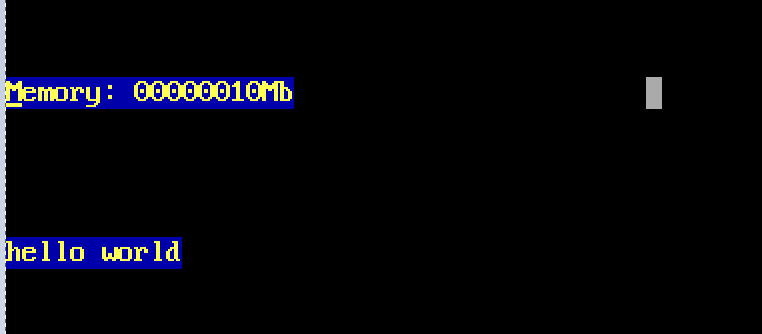
\includegraphics[width=16cm]{inc/protectedmode.png}
	\end{center}
\end{figure}





Теперь пользователь ввёл BackSpace и стёр rd. Затем пользователь нажал Shift и дописал буквы RD:

\begin{figure}[!h]
	\begin{center}
		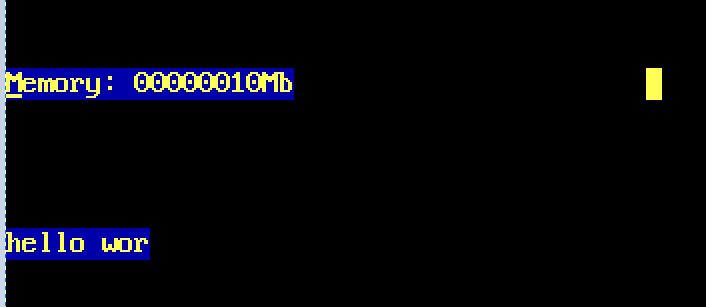
\includegraphics[width=16cm]{inc/protectedmode2.png}
	\end{center}
\end{figure}


\begin{figure}[!h]
	\begin{center}
		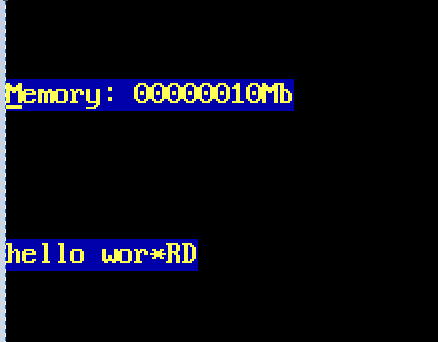
\includegraphics[width=16cm]{inc/protectedmode3.png}
	\end{center}
\end{figure}

\clearpage

Полный набор доступных символов представлен на скрине:

\begin{figure}[!h]
	\begin{center}
		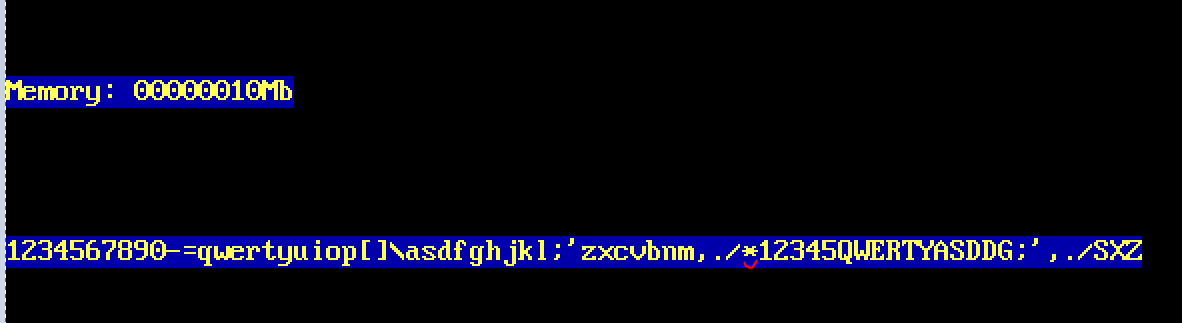
\includegraphics[width=16cm]{inc/protectedmode4.png}
	\end{center}
\end{figure}

В конце программа по нажатию Enter возвращается в реальный режим:

\begin{figure}[!h]
	\begin{center}
		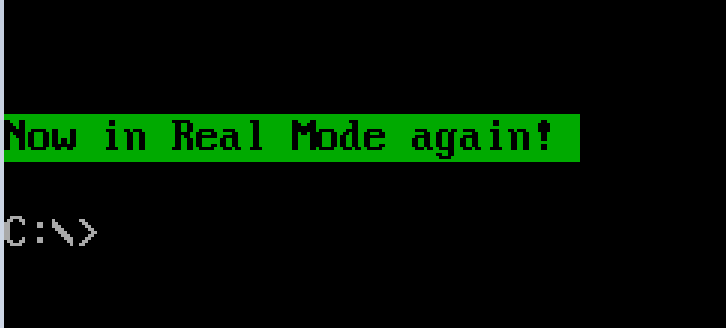
\includegraphics[width=16cm]{inc/realmode.png}
	\end{center}
\end{figure}